\documentclass[thesis.tex]{subfiles}

\chapter{Cơ sở lý thuyết và các nghiên cứu liên quan}
\section{Học máy}
Học máy là một phần trong lĩnh vực Trí Tuệ Nhân Tạo, bao gồm cung cấp kiến thức cho máy tính thông qua dữ liệu, quan sát và tương tác với thế giới (Yoshua Bengio \cite{bengio2019}). Các giải thuật Học máy sinh ra các "mô hình" từ dữ liệu trong suốt quá trình học hỏi của nó, và suy luận ra kết quả của mô hình trong suốt thời gian chạy nhằm thu được kết quả trên tập kiểm thử mà "mô hình" chưa nhìn thấy bao giờ.

Học máy hay học sâu là một lĩnh vực nằm trong lĩnh vực lớn hơn là Trí tuệ nhân tạo. Hầu hết các giải thuật học máy đều cố gắng giải quyết các tác vụ của con người, ví dụ như nhận diện thị giác, hay là đọc hiểu ngôn ngữ, vân vân,... Vì Học máy vốn là các thuật toán xấp xỉ, các bài toán đòi hỏi giải thuật Học máy thường thuộc lớp bài toán NP hoặc rất khó để tính toán.

Học máy có liên quan mật thiết đến khoa học thống kê. Một mô hình Học máy cung cấp các dự đoán dựa trên một mô hình thống kê của các dữ liệu huấn luyện. Mặc dù các mô hình tập trung vào việc tổng quát hoá những dữ liệu mới, chúng vẫn xoay quanh phân phối của tập dữ liệu huấn luyện. Hiểu rõ được các đăc điểm thống kê đối với mỗi bài toán là một bước quan trọng trong việc tạo ra các mô hình tốt.

Học máy cũng có mối quan hệ mật thiết với bài toán tối ưu: nhiều bài toán học máy được mô hình hoá như việc tối ưu hàm mất mát trên một tập dữ liệu huấn luyện. Hàm mất mát thể hiện sự khác biệt giữa kết quả dự đoán của mô hình với kết quả của dữ liệu thực tế.

Sự khác biệt chính giữa Học máy và các lĩnh vực đã đề cập ở trên nằm ở mục đích của chúng. Cả thống kê lẫn tối ưu đều tập trung vào việc trích xuất kết quả từ những dữ liệu huấn luyện đã cho, trong khi đó Học máy được nghiên cứu nhằm tổng quát hoá những dữ liệu chưa được nhìn thấy.

\subsection{Phân loại học máy}
Có nhiều loại giải thuật học máy, bao gồm: Học có giám sát, Học không giám sát, Học bán giám sát, và Học củng cố.

Các giải thuật Học có giám sát đều học từ một tập dữ liệu bao gồm cả đầu vào và đầu ra mong muốn (hay còn gọi là nhãn). Mô hình được huấn luyện bao gốm một hàm số nhằm ánh xạ bất kỳ một đầu vào cho trước nào với một đầu ra tương ứng, và nhắm vào việc xuất ra những kết quả đúng cho những dữ liệu chưa thấy và cả những dữ liệu đã thấy. Hai bài toán con của Học có giám sát là bài toán Hồi quy (với đầu ra là một giá trị liên tục) và phân lớp (với đầu ra là một hoặc nhiều giá trị rời rạc). Các giải thuật Học có giám sát phổ biến bao gồm Naive Bayes classification, \gls{svm}, Decision Trees và Neural Networks. Đây là các thuật toán phổ biến nhất trong Học máy, được sử dụng trong các lĩnh vực như bài toán phân loại ảnh, phân tích cảm giác, hay nhận diện giọng nói, vân vân,...

Các giải thuật học bán giám sát cũng tương tự, tuy nhiên chúng được thiết kế để xử lý các dữ liệu không có nhãn hoặc các tập dữ liệu rất nhỏ, bằng việc tạo ra các giả thiết heuristic cho bài toán.

Mặt khác, các giải thuật không giám sát, xử lý các dữ liệu không nhãn, chỉ biết mỗi đầu vào. Thường thì mục đích của những mô hình này là học một mối quan hệ giữa các mẫu với nhau. Thay vì trả lời phản hồi, các thuật toán học tập không được giám sát xác định các điểm chung trong dữ liệu và phản ứng dựa trên sự vắng mặt của các điểm tương đồng như vậy trong mỗi phần dữ liệu mới. Các thuật toán không giám sát phổ biến bao gồm: K-means Clustering, và Neural Autoencoders. Một ứng dụng chính của thuật toán không giám sát là phân tích cụm, các thực thể (như người dùng hay sản phẩm, vân vân,...) có thể được phân loại thành các nhóm dựa trên các đặc trưng của chúng.

Cuối cùng, các thuật toán Học tăng cường được mô hình hóa như các tác nhân trong một môi trường. Môi trường cung cấp các phản hồi tới các hành động của tác nhân, được hiểu như những giá trị phần thưởng. Mục tiêu trong Học tăng cường là học một chính sách để các tác nhân thực hiện nhằm tối ưu hoá phần thường của chúng, và hoàn thành nhiệm vụ của chúng. Các ứng dụng đáng chú ý của Học tăng cường gồm có xe tự lái và các phần mềm AI trong trò chơi (eg. Google's AlphaGo \cite{silver2016alphago}).

\subsection{Đánh đổi giữa độ thiên lệch và phương sai }
Độ thiên lệch: nghĩa là độ lệch, biểu thị sự chênh lệch giữa giá trị trung bình mà mô hình dự đoán và giá trị thực tế của dữ liệu.

Phương sai: nghĩa là phương sai, biểu thị độ phân tán của các giá trị mà mô hình dự đoán so với giá trị thực tế.

\begin{figure}[htp]
	\centering
	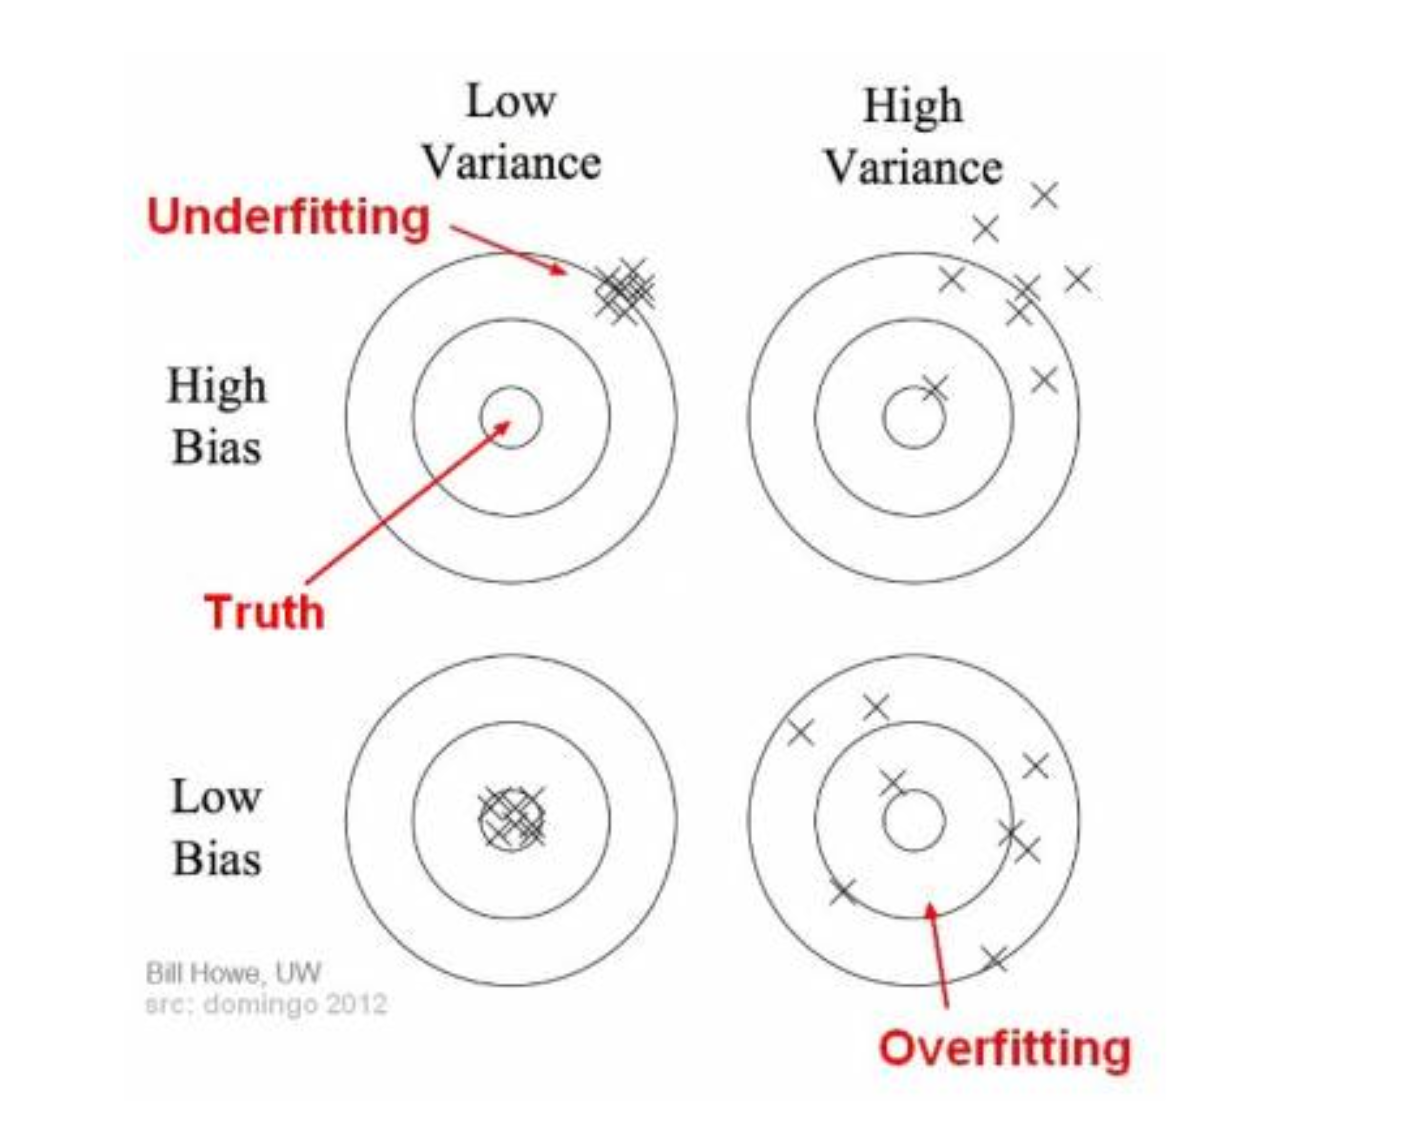
\includegraphics[width=0.7\textwidth]{bias-variance.png}
	\caption{
		Minh hoạ bias và variance)\protect\footnotemark}
	\label{fig:bias-variance}
\end{figure}
\footnotetext{https://towardsdatascience.com/understanding-confusion-matrix-a9ad42dcfd62}
\FloatBarrier

Giá trị thật dữ liệu ở giữa tâm các đường tròn. Các dấu X là các giá trị dự đoán. Ta thấy nếu bias cao thì giá trị dự đoán rất xa tâm. Tuy nhiên nếu variance cao thì các giá trị dự đoán phân tán rộng dẫn đến việc xa giá trị thực tế. Vậy nên, ta mong muốn bias thấp và variance thấp.


Nếu chúng ta biểu thị biến số mà chúng ta đang cố gắng dự đoán là Y và các hiệp biến của chúng ta là X. Ta giả sử có một mối quan hệ tương quan ví dụ như $Y=f(X)+\epsilon$ trong đó $\epsilon$ là phân phối chuẩn với kỳ vọng là không, tức là $$\epsilon \sim \mathcal{N}\left(0, \sigma_{\epsilon}\right)$$
Ta có thể ước lượng một mô hình $f \hat{(} X)$ sử dụng hồi quy tuyến tính hoặc là một kỹ thuật mô hình nào đó. Trong trường hợp này sai số bình phương kỳ vọng tại điểm $x$ là $$
\left.\operatorname{Err}(x)=E[(Y-f \hat{(} x))^{2}\right]
$$
Sai số này có thể được phân tách thành các thành phần bias và phương sai:
$$
\begin{array}{c}\operatorname{Err}(x)=(E[\hat{(x)}]-f(x))^{2}+E\left[(f \hat{(x)}-E[\hat{f}(x)])^{2}\right]+\sigma_{e}^{2} \\ \operatorname{Err}(x)=\operatorname{Bias}^{2}+\text { Variance + Irreducible Error }\end{array}
$$
Ở đây, Irreducible Error, là thuật ngữ nhiễu trong mối quan hệ thực sự mà về cơ bản không thể bị giảm bởi bất kỳ mô hình nào. Cho trước mô hình chính xác và dữ liệu không giới hạn, ta có thể giảm thiểu cả bias và phương sai về 0. Tuy nhiên thực tế thì với các mô hình chỉ gần đúng và dữ liệu hạn chế, ta cần phải đánh đỏi giữa tối ưu bias hay tối ưu phương sai.

\subsection{Phân vùng các tập dữ liệu}
Đánh giá tính hiệu quả của các mô hình Học máy khác với các mô hình và giải thuật thống kê khác. Trong phần này, chúng ta tập trung vào đánh giá các mô hình có giám sát.

Các mô hình có giám sát được huấn luyện trên tập dữ liệu huấn luyện, tuy nhiên mục tiêu nhằm xuất ra các dự đoán chính xác trên tập dữ liệu chưa nhìn thấy bên ngoài tập huấn luyện. Vì vậy ta không thể đánh giá trên dữ liệu huấn luyện. Mặt khác một mô hình mà chỉ "học" bằng việc ghi nhớ những dữ liệu huấn luyện một cách hoàn hảo thì sẽ không thể sử dụng được. Vậy nên một tập con của dữ liệu được đánh nhãn sẽ được lấy ra từ tập huấn luyện và coi đó như một tập kiểm thử mới, chỉ phục vụ cho việc đánh giá mô hình.

Thêm vào đó, có nhiều mô hình với các siêu tham số mà ta buộc phải lựa chọn dựa trên kinh nghiệm và thực nghiệm. lựa chọn này cũng nên được thực hiện trên dữ liệu không nhìn thấy, nhưng không sử dụng tập hợp thử nghiệm vì điều này chỉ đơn giản là chọn ra bất kỳ tập thông số nào xảy ra phù hợp với phân phối thử nghiệm. Thay vào đó một tập dữ liệu thẩm định sẽ được tạo ra nhằm mục đích này.

Đối với các tập dữ liệu lớn, ta thường chia tập dữ liệu theo tỷ lệ 80/20 cho huấn luyện và kiểm thử. Trong những tập dữ liệu nhỏ hơn, một hướng tiếp cận thay thế được gọi là $k$-fold cross validation, khi mà ta chia tập dữ liệu thành k phần bằng nhau được gọi là các fold. Việc huấn luyện khi đó được thực hiện $k$ lần, mỗi lần sử dụng một fold như là tập kiểm thử, và tập còn lại như là tập huấn luyện. Các kết quả đánh giá khi đó được lấy trung bình trên tất cả các lần chạy.

Khi chia các tập dữ liệu, đôi khi việc duy trì phân phối của các lớp hay các thuộc tính khác rất quan trọng trong dữ liệu gốc. Kỹ thuật này được gọi là lấy mẫu phân tầng, và đặc biệt quan trọng đối với các tập dữ liệu được phân phối không đồng đều.

Đánh giá mô hình trên nhiều tập dữ liệu khác nhau có thể bộc lộ ra nhiều những thiếu sót khác nhau. Một mô hình gọi là \textit{underfits} khi nó đạt điểm đánh giá thấp trên tập huấn luyện, điều đó có nghĩa là mô hình không thể khớp được với phân phối của dữ liệu bài toán đưa ra. Sử dụng những mô hình mạnh mẽ và phức tạp hơn có thể giải quyết được vấn đề này. Mặt khác, một mô hình gọi là \textit{overfits} khi nó đạt được điểm đánh giá cao trên tập huấn luyện, nhưng lại đạt điểm thấp trên tập thẩm định. Điều này có nghĩa rằng mô hình chỉ học được các mẫu có trong tập huấn luyện mà không phải các đặc trưng ta mong muốn. Các kỹ thuật chuẩn hoá và tăng cường dữ liệu sẽ được sử dụng nhằm cải thiện vấn đề overfitting này.

\subsection{Các độ đo đánh giá}
Các metric khác nhau được dùng để đánh giá các mô hình học máy khác nhau, tuỳ thuộc vào từng lớp bài toán. Hầu hết các metric tập trung vào việc đánh giá xem mô hình thực thi các tác vụ đã cho chính xác đến mức nào, hoặc cũng có thể bao gồm các yêu cầu khác như  tính hiệu quả, sức mạnh hay khả năng mở rộng.

Đối với các mô hình phân lớp, metric phổ biến nhất thường là để đo độ chính xác, tức là tỷ lệ giữa số mẫu được phân lớp đúng trên số mẫu mà mô hình đoán. Tuy nhiên metric này có thể bị nhiễu trên các tập dữ liệu không cân bằng. Đặc biệt, nếu như $90\%$ dữ liệu thuộc vào lớp A, thì một mô hình phân loại luôn luôn cho kết quả là lớp A sẽ đạt được $90\%$ về độ chính xác. Vậy nên, 3 metric dưới đây thường xuyên được thêm vào để đánh giá mô hình bao gồm: precision, recall và F1 score.

Precision đo tỷ lệ giữa Đúng Tích Cực (số mẫu được mô hình dự đoán chính xác cho một lớp) trên tất cả dự đoán của lớp đó. Recall đo tỷ lễ giữa Đúng Tích Cực đối với một lớp và tất cả các mẫu được gán nhãn của lớp đó. Cuối cùng, F1 score là trung bình điều hoà giữa precision và recall. Tính toán những metric này thường sử dụng một ma trận hỗn loạn để biểu diễn (Figure \ref{fig:confusion-matrix}).

\begin{figure}[htp]
	\centering
	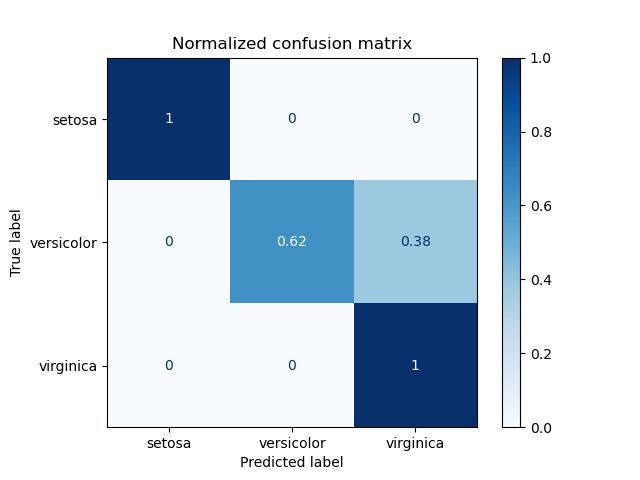
\includegraphics[width=0.5\textwidth]{confusion-matrix.png}
	\caption{
		Minh hoạ một ma trận hỗn loạn (Đúng tích cực: TP - true positive, Sai tích cực: FP - false positive, Sai tiêu cực: FN - false negative, Đúng tiêu cực: TN - true negative)\protect\footnotemark}
	\label{fig:confusion-matrix}
\end{figure}
\footnotetext{https://towardsdatascience.com/understanding-confusion-matrix-a9ad42dcfd62}
\FloatBarrier

Cụ thể ta có các công thức như dưới đây:
\begin{align}
	& Precision_i = \frac{TP_i}{TP_i + FP_i}\\
	& Recall_i = \frac{TP_i}{TP_i + FN_i}\\
	& F_1^i = 2 \frac{Precision_i \cdot Recall_i}{Precision_i + Recall_i}
\end{align}

Precision trừng phạt một mô hình khi nó đưa ra những dự đoán sai đối với một lớp cho trước, trong khi recall trừng phạt sự kém cỏi của mô hình nhằm  a model's inability to bao gồm tất cả các mẫu của lớp đó. Một mô hình mà cố gắng "gian lận" trong một metric hay lớp A model that tries to "cheat" in one metric or class (like how our hypothetical "always A" model would have perfect recall for class A) thì sẽ nhận điểm thấp trên các metric khác (ví dụ một mô hình giả định "luôn là A" thì sẽ cho recall bằng 1 đối với lớp A, nhưng precision và recall của nó đối với các lớp khác A sẽ bằng 0), khi đó thì F1 score vẫn sẽ thấp.

\section{Giới thiệu về mạng nơ-ron và học sâu}
\subsection{Các mạng nơ-ron nhân tạo và mạng kết nối đầy đủ}
Các mạng nơ-ron nhân tạo (hay được gọi tắt là mạng nơ-ron) là một lớp của các mô hình học máy được lấy cảm hứng từ các các hệ nơ-ron sinh học xử lý dữ liệu.

Mạng nơ-ron sinh học bao gồm một nhóm hoặc nhiều nhóm nơ-ron được kết nối về mặt hóa học hoặc liên kết về mặt chức năng. Một nơ-ron có thể được kết nối đến nhiều nơ-ron khác, tổng số nơ-ron và kết nối trong một mạng có thể rất lớn. Các kết nối hay còn được gọi là các khớp thần kinh, thường được cấu tạo từ sợi trục đến đuôi gai.

Các mạng nơron nhân tạo sử dụng một quy trình gần đúng được đơn giản hóa hơn nhiều, có các nơ-ron được thay thế bởi các đơn vị tính toán đơn giản nhằm thực hiện biến đổi trên dữ liệu đầu vào. Mặc dù đơn giản như vậy, nhưng với số lượng nơ-ron và kết nối lớn cho phép các mạng nơ-ron thể hiện được những hàm số cực kỳ phức tạp.

Mạng nơ-ron đầu tiên được đề xuất vào năm 1958 bởi Frank Rosenblatt \cite{rosenblatt1958perceptron}, được gọi là Perceptron. Một perceptron về cơ bản là một nơ-ron bao gồm một tập các trọng số $w$, một trọng số \textit{bias} $b$ và một hàm kích hoạt $g(x)$. Cho một vector liên tục $x$ là đầu vào, đầu ra của một perceptron được thể hiện bởi hàm sau đây:

\begin{equation}
	f(x; w, b) = g(w^T x + b)
\end{equation}

Ý tưởng của perceptron thậm chí đã được mở rộng thành perceptron đa tầng, hay còn được biết đến nhiều hơn với cái tên mạng nơ-ron nhân tạo. Nhìn chung, chúng chỉ khác ở chỗ có nhiều nơ-ron tính toán hơn thay vì chỉ có một, và chúng được chia thành các tầng khác nhau (Hình \ref{fig:nnet}).

Có 3 loại tầng được thể hiện trong một mạng nơ-ron: tầng đầu vào, các tầng ẩn và tầng đầu ra. Tầng đầu vào biểu diễn cho dữ liệu đầu vào, mỗi đơn vị chứa giá trị đặc trưng của một mẫu. Các tầng ẩn bao gồm các biến đổi được thực hiện bởi mạng trên dữ liệu đầu vào, mỗi đơn vị làm việc tương tự như một perceptron. Cuối cùng là tầng đầu ra bao gồm các giấ trị đầu ra của mạng. Cụ thể, tầng này trả về các giá trị mà ta mong muốn như là kết quả cuối cùng, hoặc là các giá trị mà có thể suy ra được kết quả cuối cùng.

\begin{figure}[htp]
	\centering
	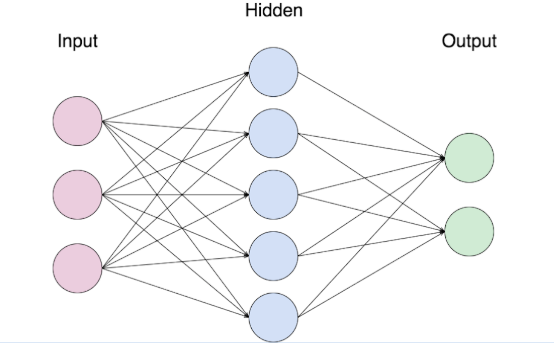
\includegraphics[width=0.5\textwidth]{nnet.png}
	\caption{Architecture of a 4-layer neural network\protect\footnotemark}
	\label{fig:nnet}
\end{figure}
\footnotetext{https://technology.condenast.com/story/a-neural-network-primer}

Trong kiến trúc này, mỗi nơ-ron trong tầng thứ $j$ được kết nối với tất cả các nơ-ron ở tầng thứ $j + 1$. Như vậy, các mạng này còn được gọi là mạng được kết nối đầy đủ.

Các mạng nơ-ron cài đặt 2 phương thức chính: Lan truyền tiến và Lan truyền ngược.

\subsubsection{Lan truyền tiến}
Lan truyền tiến được sử dụng để lấy các kết quả đầu ra từ một mạng nơ-ron. Ví dụ với đầu vào $x$ ở tầng đầu vào, chúng ta lặp qua lần lượt từng tầng một, tính toán đầu ra ở mỗi bước lan truyền (Giải thuật \ref{alg:fwd_pass}). Đầu ra cho tầng thứ $j$ được định nghĩa ở \cite{Goodfellow-et-al-2016} as:

\begin{equation}
	h^{(j)} = g^{(j)}(W^{(j)T} \cdot h^{(j-1)} + b^{(j)})
\end{equation}
Trong đó $g^{(j)}$ là hàm kích hoạt của tầng thứ $j^{th}$, $W^{(j)}$ là ma trận trọng số, $b^{(j)}$ là trọng số lệch, và $h^{(0)} = x$. Kích thước của $W^{(j)}$ tương ứng với số nơ-ron ở các tầng thứ $j$ và thứ $j - 1$.

Đối với các mạng nơ-ron được trình bày phức tạp hơn, các mô hình phi tuyến tính, hàm kích hoạt tại mỗi tầng thường là phi tuyến. Các hàm được sử dụng rộng rãi nhất là $sigmoid$ và $tanh$ (Hình \ref{fig:sigmoid-tanh}).

\begin{figure}[htp]
	\centering
	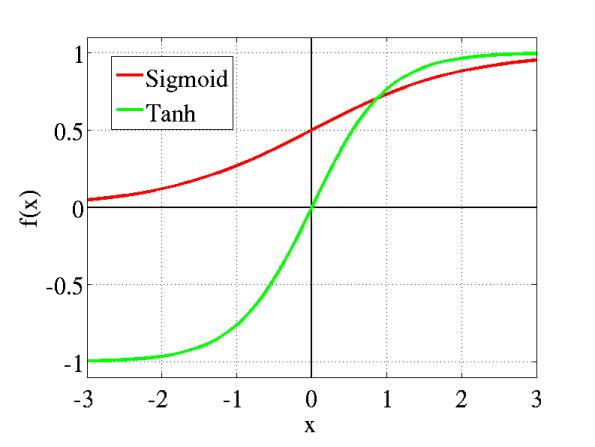
\includegraphics[width=0.5\textwidth]{images/sigmoid-tanh.png}
	\caption{Các hàm kích hoạt sigmoid và tanh\protect\footnotemark}
	\label{fig:sigmoid-tanh}
\end{figure}
\footnotetext{https://www.researchgate.net/figure/The-sigmoid-and-hyperbolic-tangent-activation-functions\_fig2\_2654867842}

\begin{algorithm}[bth]
	\SetAlgoLined
	\caption{Lan truyền tiến} \label{alg:fwd_pass}
	\Input{Vector các đặc trưng đầu vào $x$\\
		Các tầng mạng $L = ((W^{(1)}, b^{(1)}, g^{(1)}),...,(W^{(m)}, b^{(m)}, g^{(m)}))$
		}
	\Output {Các dự đoán $h^{(m)}$\\
		Đầu vào tại mỗi tầng $Z = (z^{(1)},...,z^{(m)})$
	}

	$h^{(0)} \gets x$ \\
	\For{$j \in (1...m)$} {
		$z^{(j)} \gets W^{(j)T} \cdot h^{(j-1)} + b^{(j)}$ \\
		$h^{(j)} \gets g^{(j)}(z^{(j)})$
	}

	\Return $h^{(m)}$, $Z$
\end{algorithm}

\subsubsection{Lan truyền ngược}
Các mạng nơ-ron học từ dữ liệu là dựa vào lan truyền ngược. Như tên của nó, lan truyền ngược hoạt động bằng cách truy tìm lại từ lớp đầu ra. Cho một mẫu huẫn luyện $x$ và nhãn $y$, đầu tiên chúng ta thu được dự đoán của mạng $h$ sử dụng lan truyền tiến. Ý tưởng chung là "truyền" tín hiệu lỗi giữa $h$ và $y$ tới toàn bộ mạng, hay nói cách khác, cập nhật mạng để giảm lỗi dự đoán.

Tín hiệu lỗi được tính toán sử dụng một hàm mục tiêu, đo lường sự khác biệt giữa các dự đoán và nhãn. Đặc biệt, các bài toán hồi quy sử dụng Lỗi Trung Bình Bình Phương (Công thức \ref{eq:mse}), trong khi các bài toán phân loại sử dụng hàm mất mát Cross Entropy (Công thức \ref{eq:cross_enp}). Các hàm đáng chú ý khác bao gồm Triplet Loss được dùng cho FaceNet \cite{schroff2015facenet}, và Adversarial Loss được dùng bởi các mạng học cạnh tranh \cite{goodfellow2014generative}.

\begin{align}
	& MSE = \frac{1}{n} \sum_{i=1}^n (h_i - y_i)^2 \label{eq:mse}\\
	& CE = - \frac{1}{n} \sum_{i=1}^n (y_ilog(h_i) + (1-y_i)log(1-h_i)) \label{eq:cross_enp}
\end{align}
trong đó $n$ là tổng số mẫu.

Để cập nhật mạng, chúng ta cần biết các giá trị để cập nhật từng nơ-ron. Lan truyền ngược tìm những giá trị này tại mỗi tầng $j$ sử dụng gradient w.r.t tầng thứ $j + 1$. Ta bắt đầu bằng việc tính toán gradient tại tầng đầu ra $m$ w.r.t hàm mục tiêu. Khi đó, sử dụng quy tắc chuỗi đạo hàm, tính gradient tại mỗi tầng ở trước. Mô ta chi tiết trong thuật toán \ref{alg:backprop}.

\begin{algorithm}[bth]
	\SetAlgoLined
	\caption{Backpropagation} \label{alg:backprop}
	\Input{Vector of input features $x$\\
		Ground truth labels $y$\\
		Network layers $L = ((W^{(1)}, b^{(1)}, g^{(1)}),...,(W^{(m)}, b^{(m)}, g^{(m)}))$
		}
	\Output {Gradients at each layer $\Delta = (\delta^{(1)},...,\delta^{(m)})$
	}

	$h, Z \gets forwardPass(x)$ \\
	$c \gets loss(h, y)$ \\
	$\delta^{(m)} = \frac{\delta c}{\delta W^{(m)}} \odot g^{(m)'}(z^{(m)})$ \\
	\For{$j \in (m-1...1)$} {
		$\delta^{(j)} \gets (W^{(j+1)T} \cdot \delta^{(j+1)}) \odot g^{(j)'}(z^{(j)})$
	}

	\Return $\Delta$
\end{algorithm}
\FloatBarrier

\subsubsection{Thuật toán xuống dốc}
Với gradient tại mỗi tầng, ta có thể cập nhật mạng bằng cách "di chuyển" trong các hướng đối nhau của vector đạo hàm. Với một bước đủ nhỏ, ta có thể đảm bảo rằng hàm mục tiêu giảm. Bằng việc lặp lại thủ tục này trong tập huấn luyện, mạng có thể hội tụ về mức tối thiểu của hàm mất mát. Thủ tục này được gọi là thuật toán xuống dốc (Giải thuật \ref{alg:grad_desc}).

\begin{algorithm}[bth]
	\SetAlgoLined
	\caption{Thuật toán xuống dốc} \label{alg:grad_desc}
	\Input{Vector đặc trưng đầu vào $x$\\
		Các nhãn thật $y$\\
		Các tầng mạng $L = ((W^{(1)}, b^{(1)}, g^{(1)}),...,(W^{(m)}, b^{(m)}, g^{(m)}))$\\
		Tỷ lệ học $\gamma$
		}
	\Output {Mạng được cập nhật}
	
	\Repeat{Hội tụ} {
		$\Delta \gets backprop(x, y, L)$ \\
		\For{$j \in (1...m)$} {
			$W^{(j)} \gets W^{(j)} - \gamma \delta^{(j)}$
		}
	}
\end{algorithm}
\FloatBarrier

Tốc độ học được dùng để điều chỉnh bước cho mỗi lần thuật toán xuống dốc tại mỗi vòng lặp. Tốc độ học cao có nghĩa là mạng được cập nhật với những bước rộng, làm cho nó dễ bị phân kỳ ở các bước sau. Tốc độ học thấp thì sẽ đảm bảo hơn về sự hội tụ, nhưng sẽ tốn nhiều thời gian hơn. Thông thường thì tốc độ học nằm trong khoảng từ $10^{-2}$ đến $10^{-5}$.

\begin{figure}[htp]
	\centering
	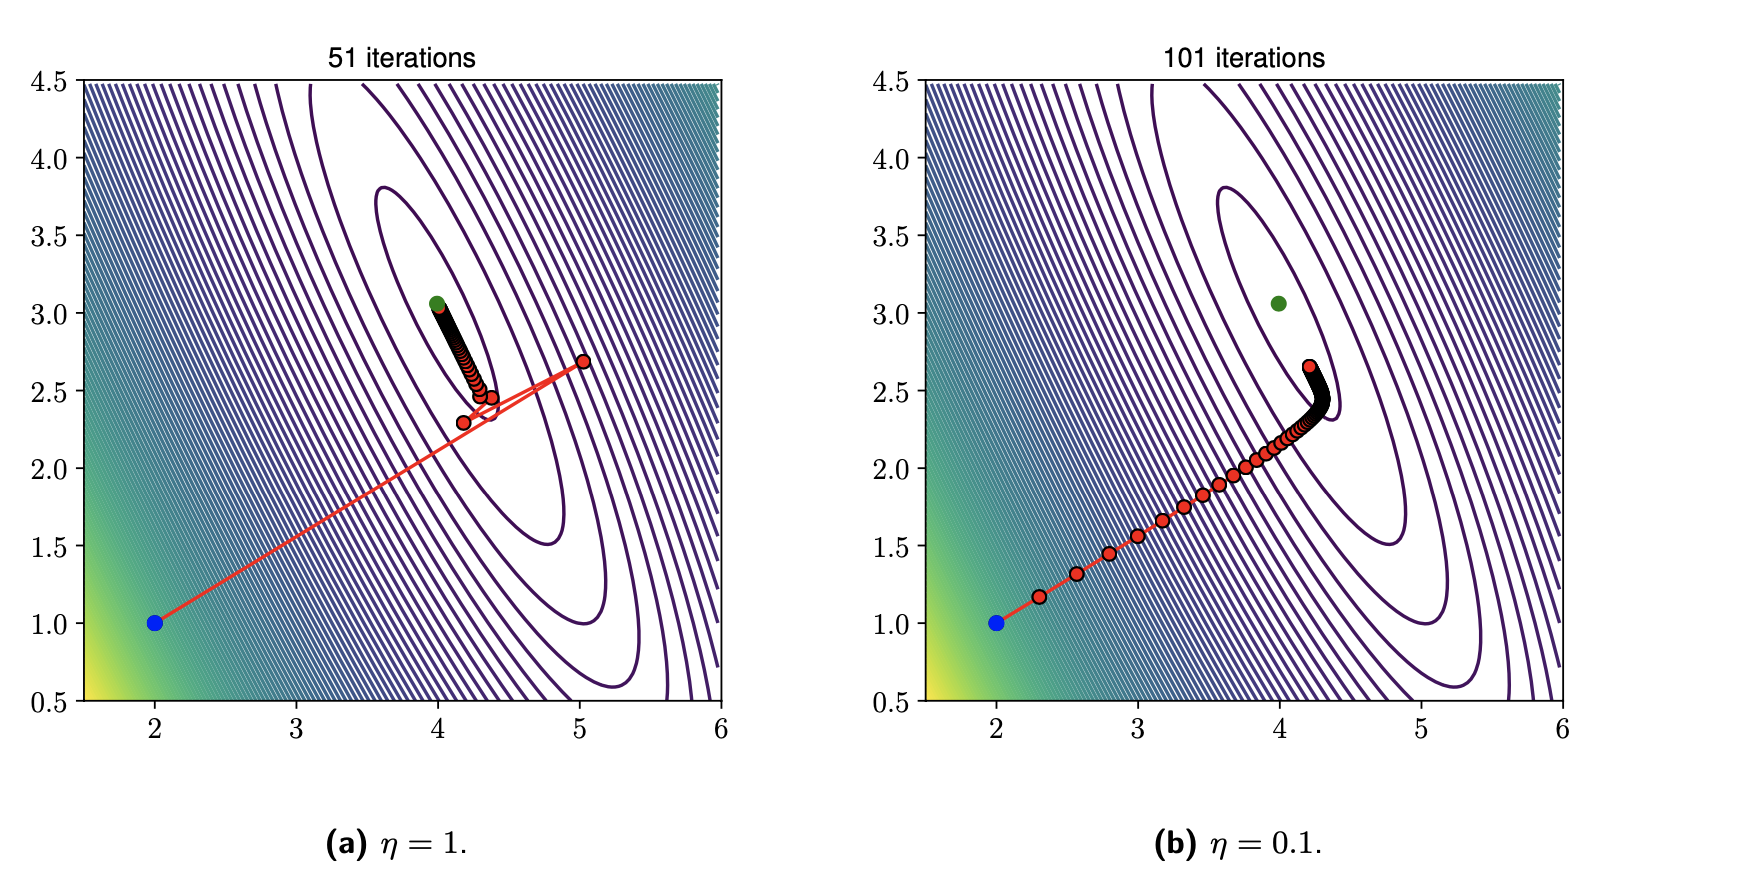
\includegraphics[width=0.6\textwidth]{gradient_descent.png}
	\caption{Đường đi nghiệm của linear regression với các learning rate khác nhau\protect\footnotemark}
	\label{fig:gradient_descent}
\end{figure}
\FloatBarrier
\footnotetext{Machine Learning cơ bản - Vũ Hữu Tiệp}

Gradient descent tính đạo hàm trên toàn bộ tập dữ liệu. Đối với những tập dữ liệu rất lớn thì không khả thi cho lắm. Minibatch gradient descent là một phiên bản chỉnh sửa chỉ cập nhật mô hình trên một vài mẫu tại một thời điểm (1 batch). Phiên bản này chạy nhiều "vòng", mỗi vòng chạy qua tất cả các batch trong tập dữ liệu. Stochastic gradient descent (SGD) \cite{bottou2012stochastic} là một biến thể với kích thước batch là 1. Stochastic và minibatch gradient descent thường đòi hỏi tốc độ học thấp hơn và nhiều vòng lặp hơn, nhưng vẫn hội tụ tại điểm cần với bộ nhớ thấp hơn.

% \begin{figure}[htp]
% 	\centering
% 	\includegraphics[width=0.7\textwidth]{gradient_descent_2.png}
% 	\caption{Convergence comparison of different gradient descent versions\protect\footnotemark}
% 	\label{fig:gradient_descent_2}
% \end{figure}
% \footnotetext{https://towardsdatascience.com/gradient-descent-algorithm-and-its-variants-10f652806a3}

Ngoài ra, rất nhiều nghiên cứu đã được thực hiện về việc điều chỉnh tỷ lệ học trong quá trình huấn luyện, đáng chú ý nhất một số thuật toán tối ưu như Adam \cite{kingma2014adam}, Adadelta \cite{zeiler2012adadelta} và RMSprop \cite{tieleman2014rmsprop}.

Nhìn chung, các mạng càng nhiều tầng và nơ-ron thí càng khớp hơn với dữ liệu huấn luyện. Tuy nhiên, không phải lúc nào tăng số nơ-ron cũng làm tăng độ chính xác. Các mạng nơ-ron lớn thì lại bị quá khớp rất nhanh, trong khi các mạng sâu hơn 5 - 6 lớp bị biến mất đạo hàm. Bởi vì những giới hạn này, kiến trúc mạng nơ-ron truyền thống chỉ khả thi ở một kích thước nhất định.

Các kỹ thuật Học sâu cố gắng tạo ra các mạng lớn hơn và sâu hơn để vượt qua những thách thức này. Các kỹ thuật này bao gồm các mạng, thuật toán tối ưu, các hàm kích hoạt,... Trong phần tiếp theo, chúng ta sẽ xem xét Mạng nơ-ron tích chập, một trong những mô hình có tác động mạnh nhất trong Học sâu.

\subsection{Mạng nơ-ron tích chập}
Mạng nơ-ron tích chập (Convolutional Neural Network \cite{kim2017convolutional} - \gls{cnn}) ban đầu được thiết kế nhằm mục đích xử lý ảnh. Các kiến trúc của chúng hướng tới một vẫn đề cốt lõi khi sử dụng mạng nơ-ron để xử lý ảnh đó là kích thước đầu vào có thể rất lớn ( ví dụ 200 x 200 x 3) sẽ làm tăng chi phí tính toán với mạng quá đơn giản và dễ gây overfit dữ liệu.

Một mạng \gls{cnn} truyền thống được cấu thành từ các thành phần sau:

Tầng Đầu vào cũng giống với mạng kết nối đầy đủ, giữ được các đặc trưng của đầu vào.

Tầng tích chập là lõi của một mạng tích chập (Hình \ref{fig:conv}). Các tham số của nó bảo gồm một tập các bộ lọc có thể học được. Các bộ lọc nhỏ (với chiều rộng và chiều cao nhỏ), nhưng mở rộng về mặt chiều sâu của dữ liệu đầu vào. Ví dụ, một bộ lọc phổ biến trên tầng đầu tiên của một mạng tích chập có thể có kích thước là 5x5x3 (i.e. 5 điểm ảnh chiều rộng, 5 điểm ảnh chiều cao và 3 kênh màu sắc). Trong suốt giai đoạn chuyển tiếp, ta trượt bộ lọc theo chiều dọc và chiều cao của ảnh đầu vào rồi tính các tích điểm ảnh tương ứng giữa bộ lọc và ảnh đầu vào ở mỗi vị trí. Khi bộ lọc trượt qua ảnh đầu vào, nó xuất ra một đồ thị kích hoạt 2 chiều thể hiện phản hồi của nó tại mỗi vị trí không gian. mạng sẽ tìm hiểu các bộ lọc kích hoạt khi chúng nhìn thấy một số đặc trưng trực quan như là cạnh của một số hướng hay là một vết màu, hay là các mẫu hình phức tạp trên các tầng cao hơn của mạng. Đồ thị kích hoạt từ các bộ lọc khác nhau được xếp chồng lên nhau dọc theo kích thước chiều sâu và tạo ra kết quả đầu ra.

\begin{figure}[htp]
	\centering
	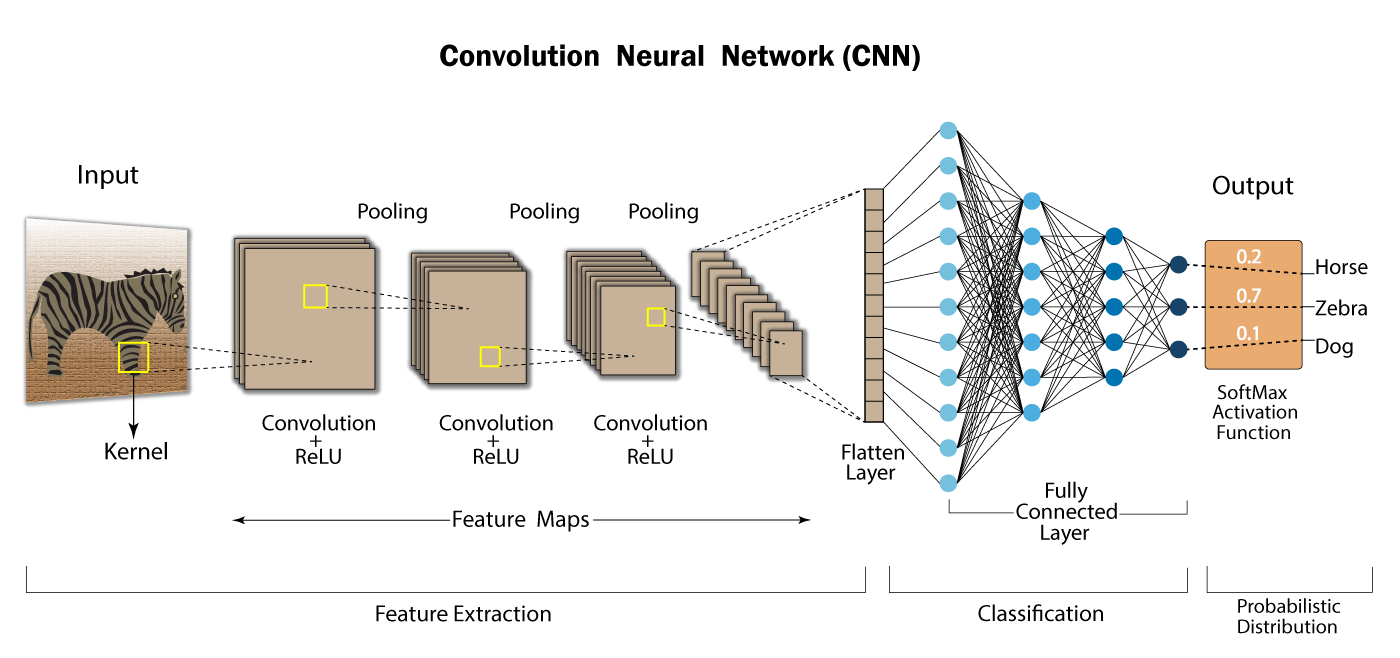
\includegraphics[width=0.6\textwidth]{conv.png}
	\caption{An example convolution layer\protect\footnotemark}
	\label{fig:conv}
\end{figure}
\footnotetext{http://cs231n.github.io/understanding-cnn/}

Một khác biệt chính giữa các tầng CONV và các tầng ẩn phổ biến nằm ở các kết nối địa phương của chúng. Mỗi nơ-ron chỉ được kết nối với một vùng địa phương của ảnh được cho vào mô hình. Phạm vi không gian của kết nối này là một siêu tham số được gọi là trường tiếp nhận (hay kích thước bộ lọc). Mức độ kết nối dọc theo độ sâu luôn bằng với độ sâu của dữ liệu đầu vào. Cần nhấn mạnh sự bất đối xứng này trong cách chúng ta xử lý các chiều không gian khác nhau (chiều rộng, chiều cao và chiều sâu): Các kết nối không gian mang tính địa phương nhưng luôn phải đầy đủ dọc theo toàn bộ dữ liệu đầu vào.

Giả định được thực hiện bởi phép tích chập là nếu một đặc trưng là một đại diện tốt đối với một vùng ảnh, thì nó cũng có thể tốt cho các vùng khác. Khi các bộ lọc thực hiện phép toán tích chập, cách sử dụng các trọng số là như nhau, và gradient của chúng tích tụ trong suốt quá trình lan truyền ngược. Điều này cho phép các tầng tích chập chia sẻ trọng số giữa các vùng ảnh, làm giảm đáng kể kích thước của chúng trong khi vẫn đảm bảo toàn bộ dữ liệu đầu vào.

Thay cho các hàm kích hoạt như là $sigmoid$ hay $tanh$, các tầng tích chập thường được kích hoạt bởi hàm ReLU, với $ReLU(x) = max(x, 0)$. ReLU có một vài thuộc tính có thể giúp ích cho những mạng rất sâu:

\begin{itemize}
	\item ReLU là hàm phi tuyến tính 
	\item Đạo hàm của ReLU bằng 1 hoặc 0, có nghĩa rằng nó không bị ảnh hưởng bởi sự mất mát đạo hàm 
\end{itemize}

Một nhược điểm của hàm ReLU là sự tồn tại của "tế bào thần kinh chết" có đầu ra là âm. Những nơ-ron này sẽ có đạo hàm bằng 0 và không thể học hoặc đóng góp vào mạng. Các hàm thay thế khác như Leaky ReLU hay Exponential ReLU đã được đề xuất để giải quyết vấn đề này.

Các lớp POOL (pooling) được sử dụng để giảm dần kích thước không gian của biểu diễn nhằm giảm lượng tham số và tính toán trong mạng, từ đó cũng giúp kiểm soát overfit. Lớp POOL hoạt động độc lập trên mọi lát cắt sâu của đầu vào và thay đổi kích thước của nó theo không gian, sử dụng toán tử MAX. Phổ biến nhất là tầng pooling với các bộ lọc 2x2 được áp dụng với sải bước bằng 2 làm giảm chiều mỗi lát cắt theo chiều sâu trong dữ liệu đầu vào theo cả chiều rộng và chiều cao, loại bỏ 75\% các hàm kích hoạt. Mỗi toán tử MAX sẽ lấy giá trị lớn nhất trong 4 giá trị (nằm trong vùng 2x2 của bộ lọc). Kích thước chiều sâu vẫn không thay đổi (Hình \ref{fig:maxpool}).

\begin{figure}[htp]
	\centering
	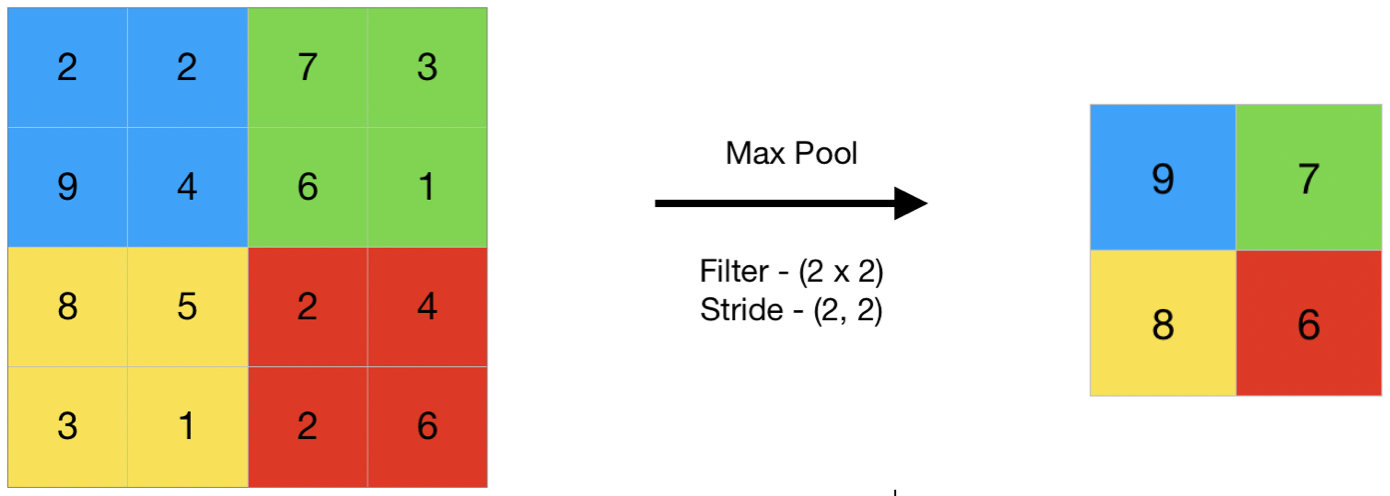
\includegraphics[width=0.6\textwidth]{maxpool.png}
	\caption{Một ví dụ về maxpooling\protect\footnotemark}
	\label{fig:maxpool}
\end{figure}
\footnotetext{http://cs231n.github.io/understanding-cnn/}

Hơn nữa để dùng max pooling, các đơn vị pooling cũng có thể thực hiện các hàm khác nhau ví dụ như pooling trung bình hoặc pooling L2-norm. Trước đây pooling trung bình thường được sử dụng nhiều nhưng gần đây không còn được ưa chuộng như toán tử max pooling đang thể hiện sự vượt trội trong thực nghiệm.

Các mạng \gls{cnn} được cấu thành từ các "khối" CONV, ReLU, POOL với các kích thước khác nhau, và cuối cùng được gắn thêm một vài tầng kết nối đầy đủ để sinh ra các kết quả phân loại cần thiết. VGGNet \cite{Simonyan14c} là một mạng rất phổ biến trong các kiến trúc như thế này.

Các kiến trúc được giới thiệu sau thường phức tạp hơn, các thứ tự phi tuyến tính của các khối tích chập để tăng khả năng học hỏi của mạng. Ví dụ như ResNet \cite{he2016resnet} sử dụng các kết nối bỏ qua (thường được gọi là các "khối dư") giữa các khối tích chập.

\subsection{Hàm mục tiêu và giải thuật huấn luyện}

\subsubsection{Cross Entropy Loss}
Cross Entropy Loss \cite{zhang2018generalized} là hàm mục tiêu được sử dụng phổ biến nhất cho các bài toán phân loại ảnh pixel-wise cross entropy. Hàm mục tiêu này kiểm tra từng pixel riêng lẻ, so sánh các dự đoán của lớp (vector pixel theo chiều sâu) với vector mục tiêu được mã dưới dạng one-hot (vector chỉ có các giá trị 0 và 1).

\begin{figure}[htp]
	\centering
	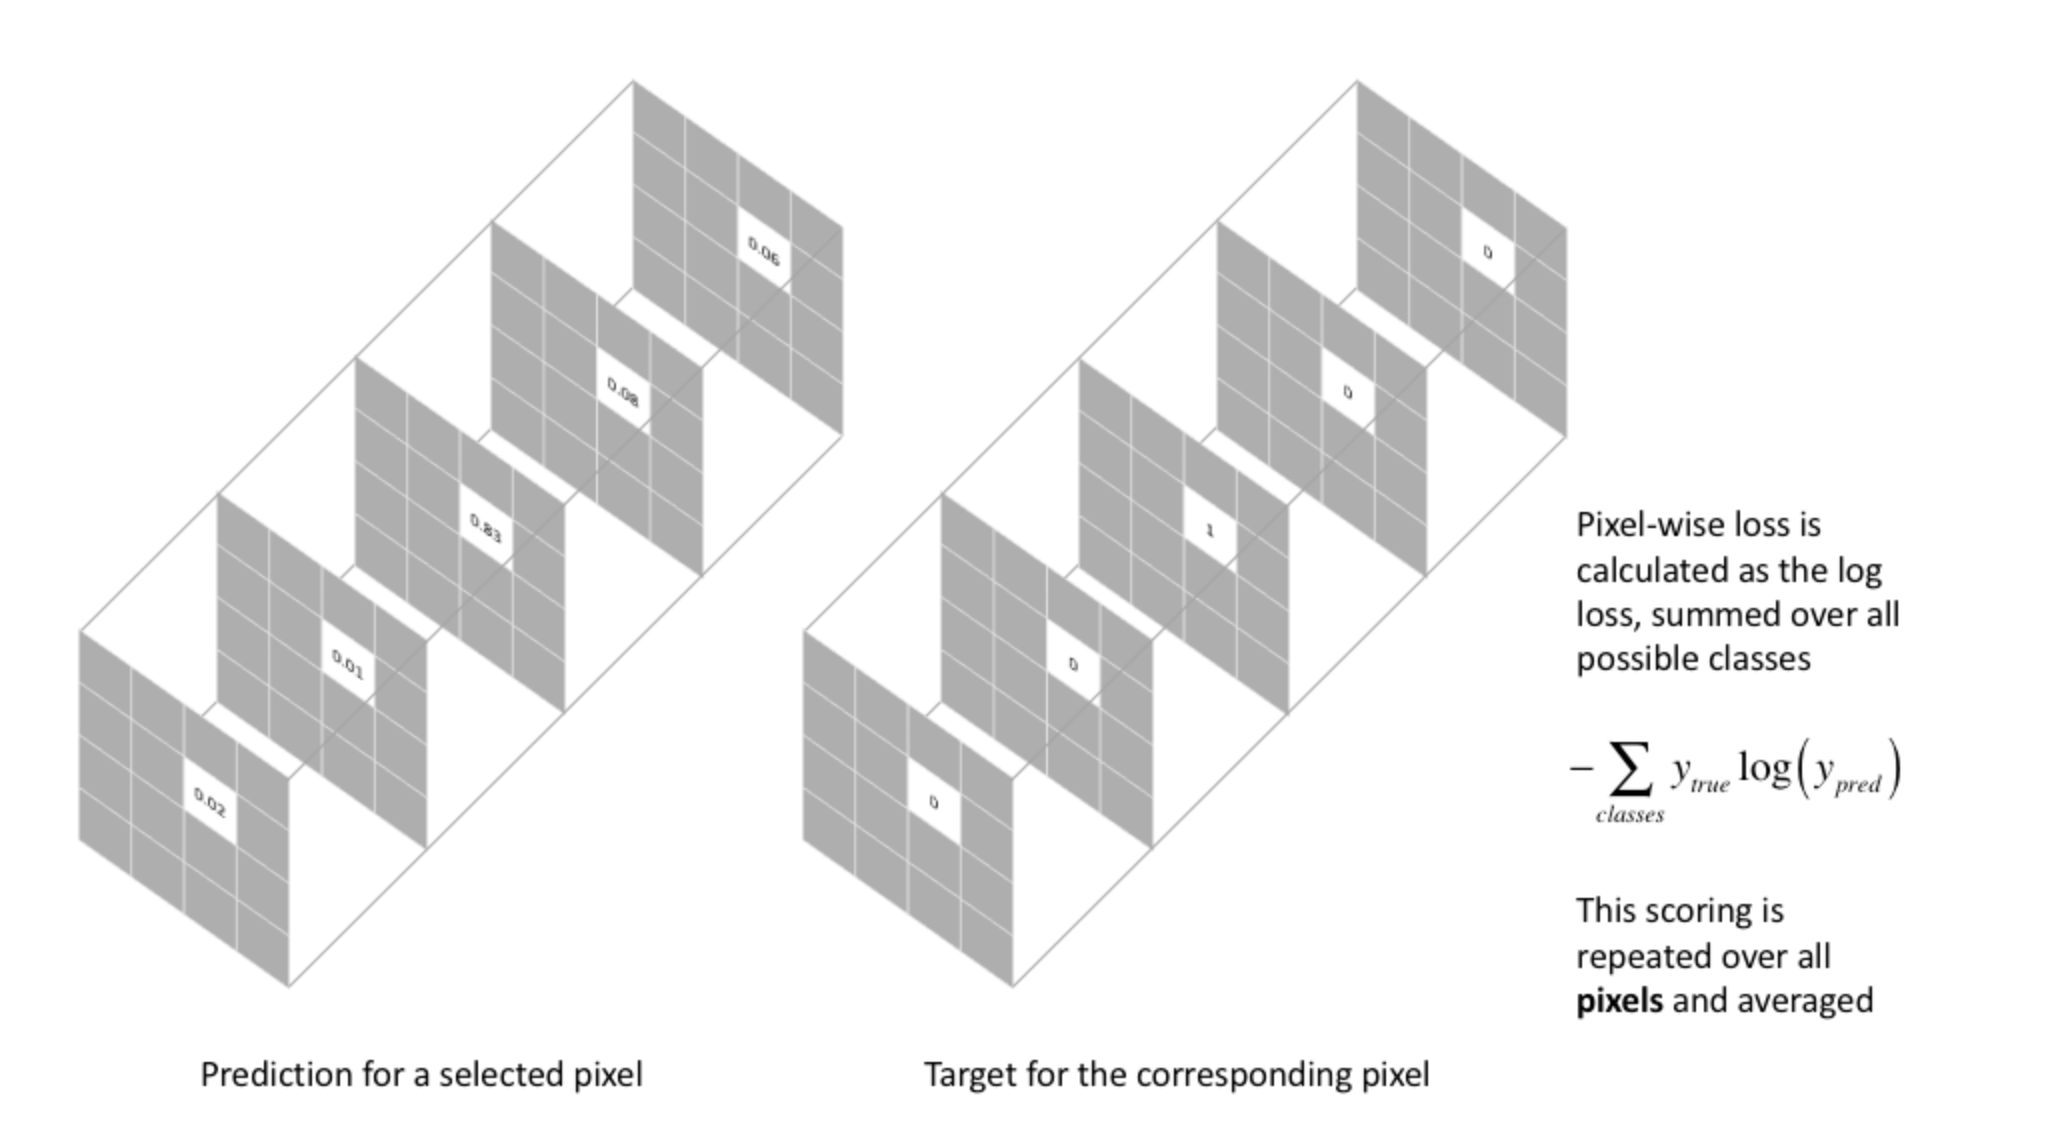
\includegraphics[width=0.6\textwidth]{images/crossentropy.png}
	\caption{Minh hoạ cho cách dùng cross entropy \protect\footnotemark}
	\label{fig:crossentropy}
\end{figure}
\footnotetext{https://www.jeremyjordan.me/semantic-segmentation/}

Bởi vì hàm cross entropy đánh giá các dự đoán lớp đối với mỗi điểm ảnh một cách độc lập và sau đó tính trung bình tất cả các điểm ảnh. Vậy nên về cơ bản thì việc học là bình đẳng giữa các điểm ảnh trong hình. Đây có thể là một vấn đề nếu các lớp khác nhau của bài toán có biểu diễn không cân bằng trong hình ảnh, khi huấn luyện có thể bị chi phối bởi lớp xuất hiện nhiều nhất. Hệ số xúc xắc ban đầu vốn được phát triển cho dữ liệu nhị phân và có thể tính được bởi công thức sau: 

$$
\text { Cross Entropy }=-\frac{1}{N} \sum_{j} y_{j} * \log \left(\widehat{y_{j}}\right)
$$
Trong đó, $y_{j}$ là nhãn thật, $\widehat{y_{j}}$ là nhẵn dự đoán


\subsubsection{Dice Loss}

Dice Loss \cite{sudre2017generalised} là một hàm mục tiêu phổ biến khác cho các bài toán phân vùng ảnh là dự trên hệ số xúc xắc, vốn là một phép đo cơ bản cho mức độ chồng chéo giữa hai mẫu với nhau. Số đo này nằm trong khoảng từ 0 đến 1 trong đó hệ số Xúc xắc thể hiện cho sự chồng chéo hoàn hảo và hoàn chỉnh. 

\begin{align}
& Dice =\frac{2|A \cap B|}{|A|+|B|}
\end{align}

Trong đó $A \cap B$ thể hiện tập các phần tử chung giữa A và B, $|A|$ thể hiện các phần tử thuộc A (tương tự với B).

Lấy ví dụ về hệ số xúc xắc trên mặt nạ phân vùng được dự đoán, ta xấp xỉ $|A \cap B|$ như là phép nhân từng phần tử tương ứng giữa dự đoán của mô hình với mặt nạ mục tiêu rồi sau đó cộng tổng ma trận kết quả. 

\begin{figure}[htp]
	\centering
	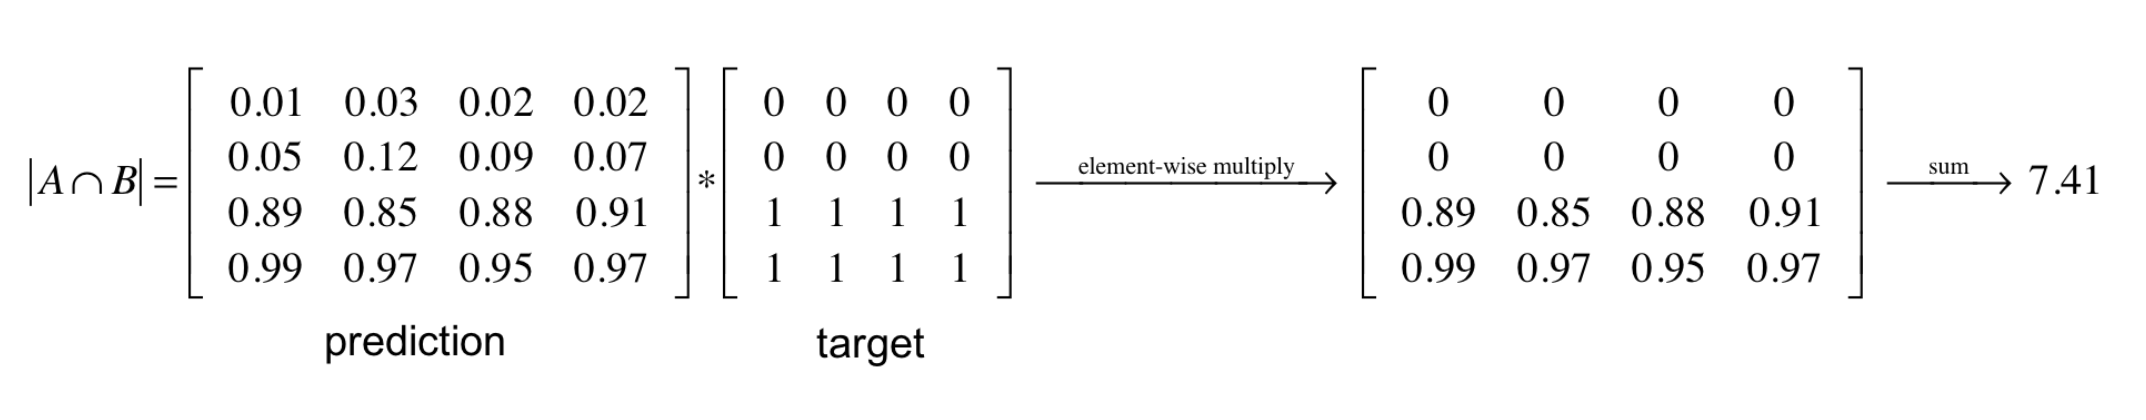
\includegraphics[width=0.8\textwidth]{images/elemenwise.png}
	\caption{Phép nhân tương ứng từng điểm ảnh rồi cộng tổng kết quả thu được \protect\footnotemark}
	\label{fig:elemenwise}
\end{figure}
\footnotetext{https://www.jeremyjordan.me/semantic-segmentation/}

Bởi vì các mặt nạ của ta là nhị phân, nên ta có thể loại bỏ một cách hiệu quả bất kỳ điểm ảnh nào mà không "hoạt động" trong mặt nạ mục tiêu khỏi dự đoán của mình. Đối với những điểm ảnh còn lại, về căn bản thì ta sẽ trừng phạt các dự đoán có độ tin cậy thấp; với một giá trị cao hơn thì sẽ dẫn tới hệ số xúc xắc tốt hơn. 

Để định lượng $|A|$ và $|B|$, đơn giản ta chỉ cộng tổng bình phương các điểm ảnh. Ta có hình \ref{fig:sumsquare} 
\begin{figure}[htp]
	\centering
	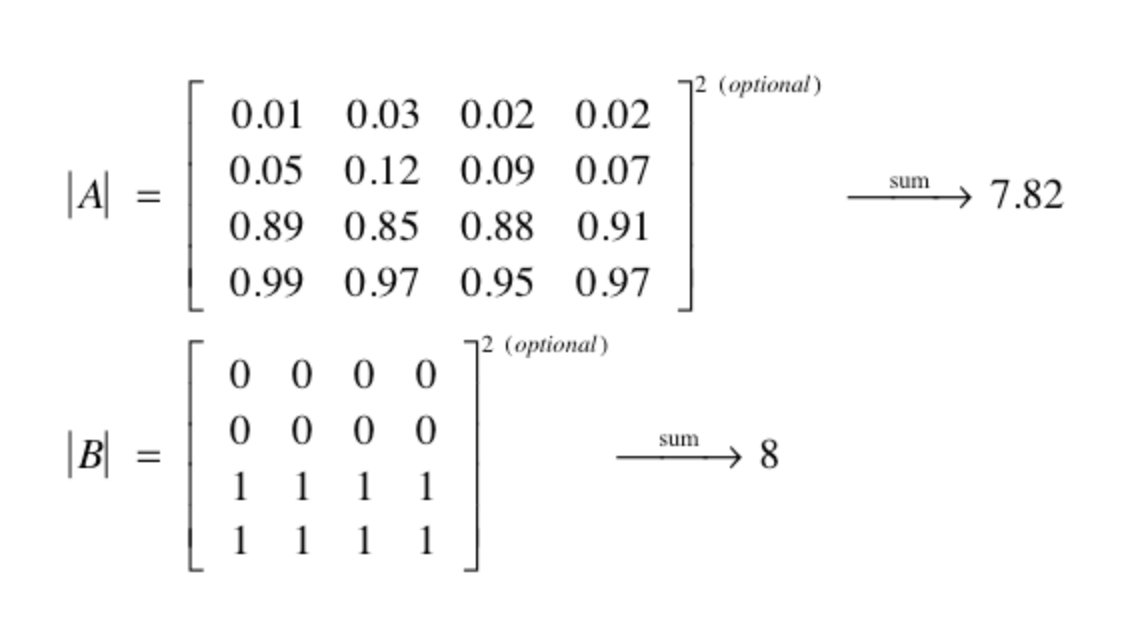
\includegraphics[width=0.8\textwidth]{images/sumsquare.png}
	\caption{Tổng các bình phương điểm ảnh định lượng cho tập A và tập B \protect\footnotemark}
	\label{fig:sumsquare}
\end{figure}

Có 2 ở tử số khi ta tính hệ số xúc xắc vì mẫu số của chúng ta "đếm gấp đôi" các phần tử chung giữa hai tập. Để tính một hàm mục tiêu mà có thể được tối ưu, ta sử dụng 1 - Dice. Hàm mục tiêu này được biết đến như là "Hàm xúc xắc mềm" bởi vì ta sử dụng các xác suất được dự đoán thay vì dùng ngưỡng và biến chúng thành mặt nạ nhị phân. 

Đối với đầu ra của hàm nơ-ron, tử số liên quan đến các kích hoạt chung giữa dự đoán của mô hình và mặt nạ mục tiêu, trong đó mẫu số liên quan đến số lượng kích hoạt trong mỗi mặt nạ riêng biệt. Điều này có tác dụng chuẩn hoá mất mát theo kích thước của mặt nạ mục tiêu để "hàm mục tiêu xúc xắc mềm" không gặp khó khăn trong việc học từ các lớp có ít biểu diễn không gian hơn trong một hình ảnh. 

\begin{figure}[htp]
	\centering
	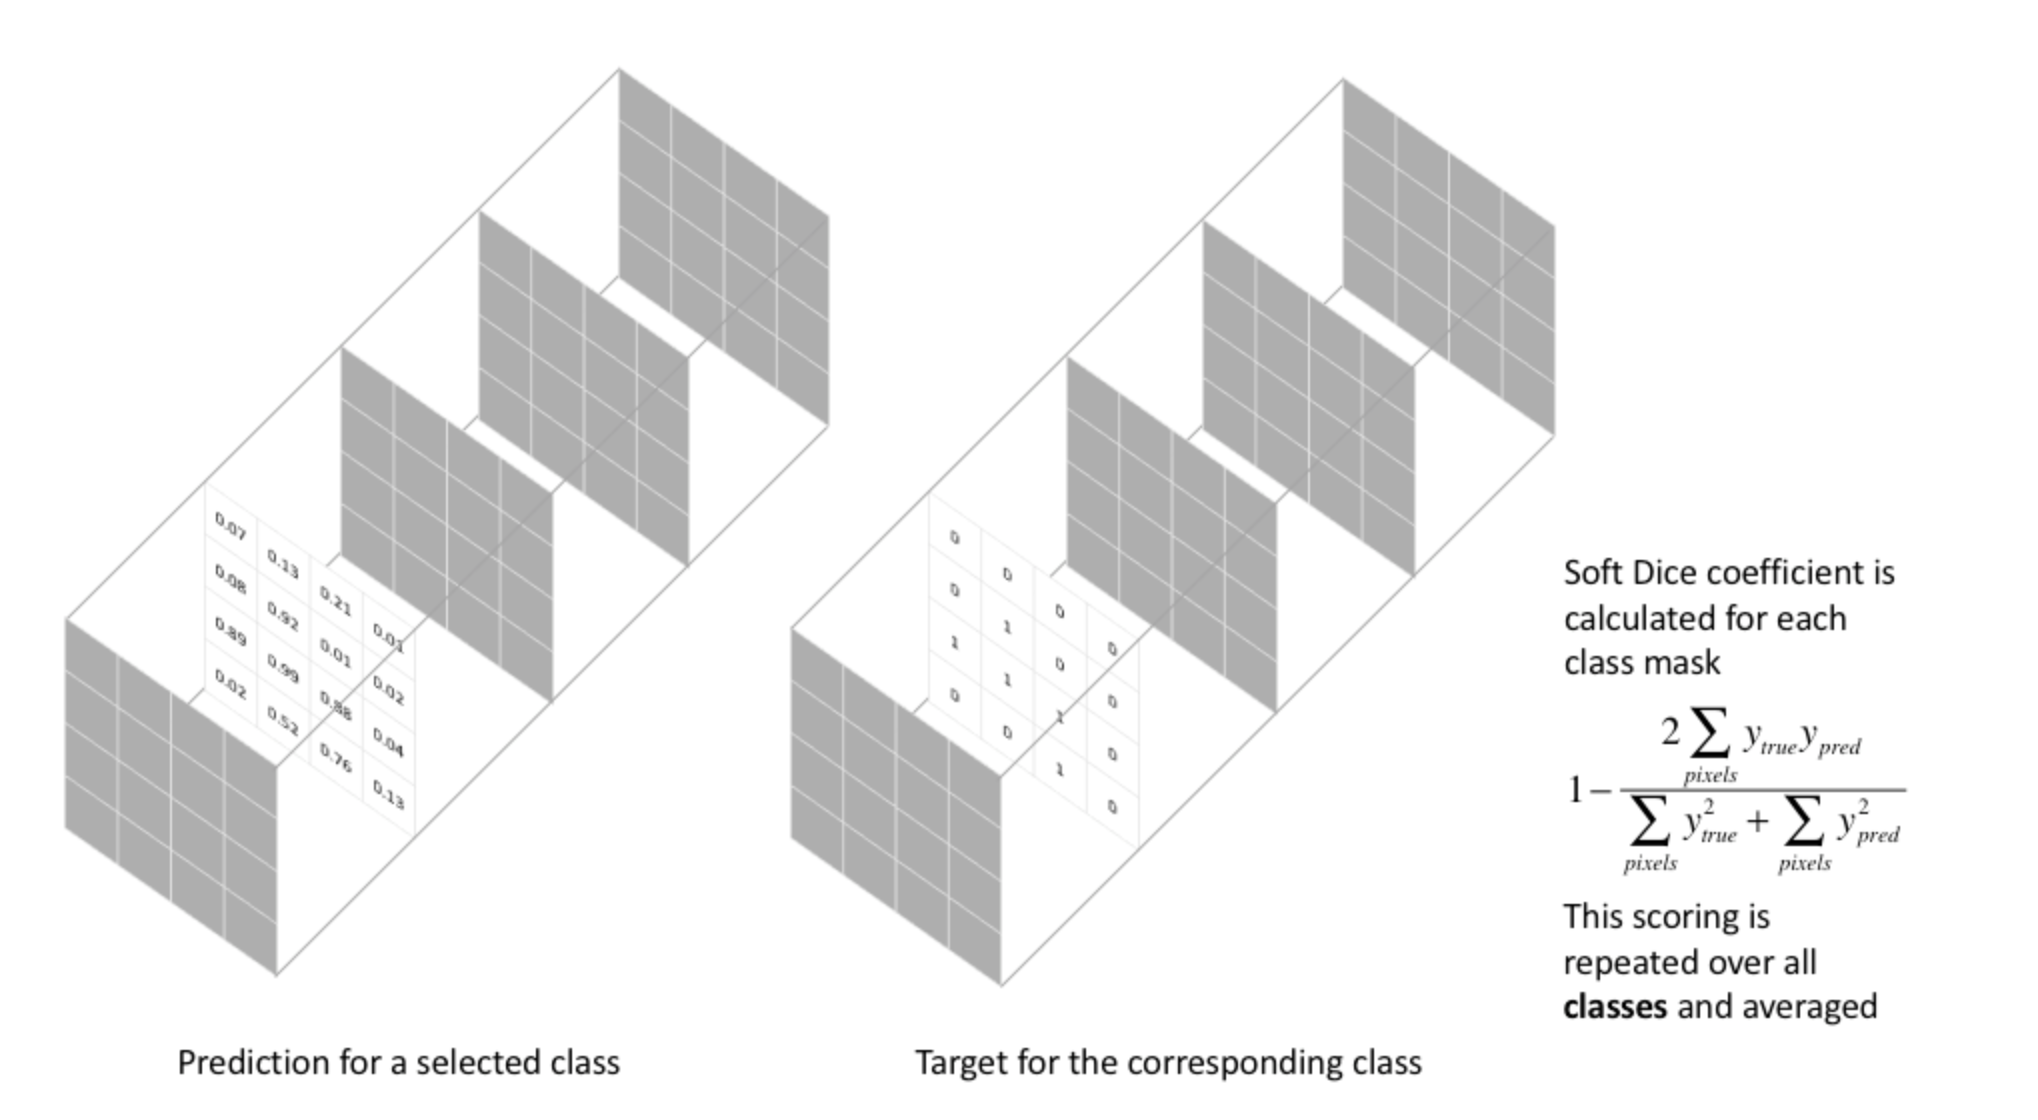
\includegraphics[width=0.8\textwidth]{images/diceloss.png}
	\caption{ Một hàm mất mát xúc xắc mềm được tính cho từng lớp riêng biệt và sau đó lấy trung bình cộng để thu được kết quả cuối cùng \protect\footnotemark}
	\label{fig:diceloss}
\end{figure}